\section{qtgraph.\-cpp File Reference}
\label{qtgraph_8cpp}\index{qtgraph.\-cpp@{qtgraph.\-cpp}}
{\ttfamily \#include $<$qapplication.\-h$>$}\\*
{\ttfamily \#include $<$qwidget.\-h$>$}\\*
{\ttfamily \#include $<$qlabel.\-h$>$}\\*
{\ttfamily \#include $<$qpainter.\-h$>$}\\*
{\ttfamily \#include $<$q3picture.\-h$>$}\\*
{\ttfamily \#include $<$Q\-Palette$>$}\\*
{\ttfamily \#include $<$Q\-Mouse\-Event$>$}\\*
{\ttfamily \#include $<$Q\-Paint\-Event$>$}\\*
{\ttfamily \#include $<$Q\-Image\-Writer$>$}\\*
{\ttfamily \#include $<$malloc.\-h$>$}\\*
{\ttfamily \#include $<$iostream$>$}\\*
{\ttfamily \#include $<$qtimer.\-h$>$}\\*
{\ttfamily \#include $<$qpixmap.\-h$>$}\\*
{\ttfamily \#include $<$qimage.\-h$>$}\\*
{\ttfamily \#include $<$q3strlist.\-h$>$}\\*
{\ttfamily \#include $<$Q\-Resize\-Event$>$}\\*
{\ttfamily \#include \char`\"{}qtgraph.\-h\char`\"{}}\\*
{\ttfamily \#include \char`\"{}parameter.\-h\char`\"{}}\\*
Include dependency graph for qtgraph.\-cpp\-:
\nopagebreak
\begin{figure}[H]
\begin{center}
\leavevmode
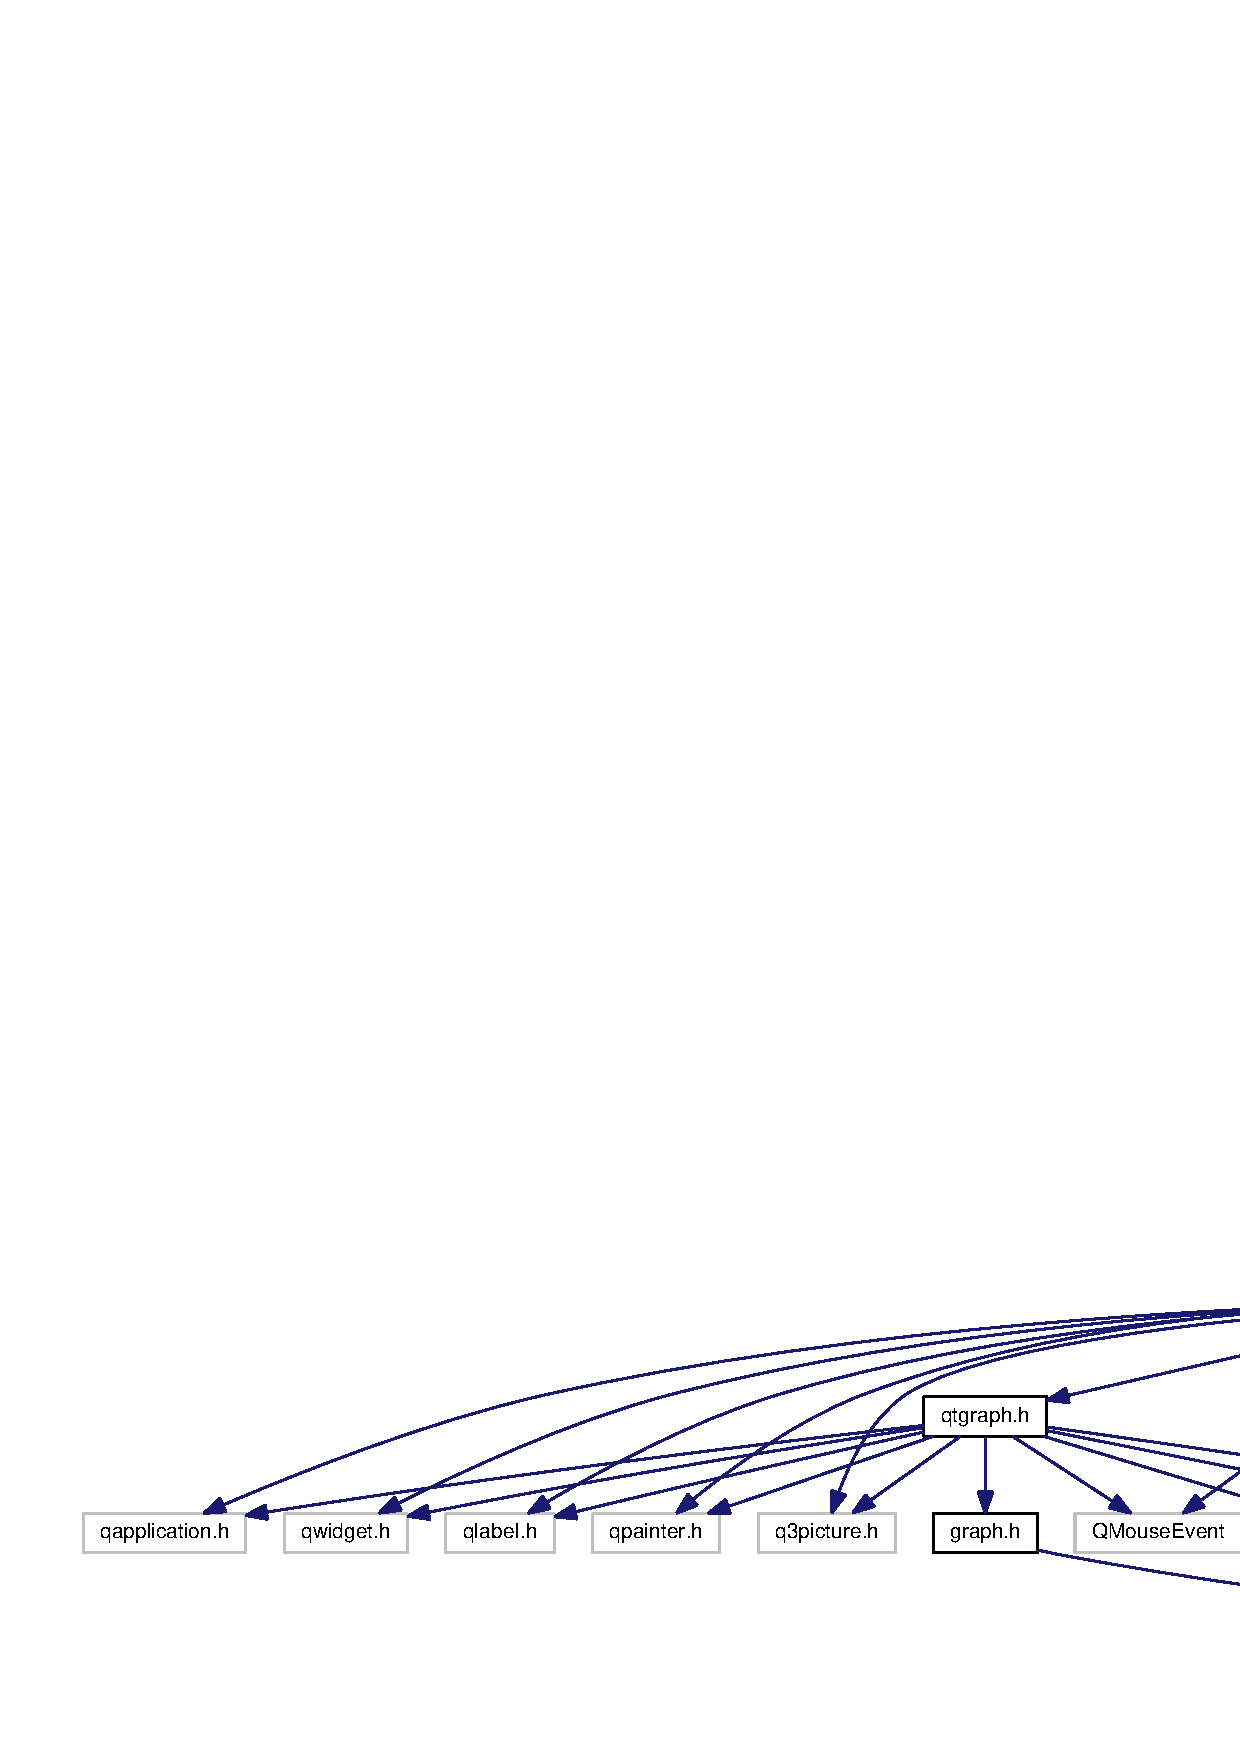
\includegraphics[width=350pt]{qtgraph_8cpp__incl}
\end{center}
\end{figure}
